\documentclass[aspectratio=169]{beamer}
\setbeamertemplate{navigation symbols}{}
\usepackage{color, amsmath, comment, subfigure}
\usepackage{url}

\usepackage{hyperref}
\hypersetup{
    colorlinks=true,
    linkcolor=blue,
    filecolor=magenta,      
    urlcolor=cyan,
}

%%%%%%%%%%%%%%%%%%%%%%%%%%
\title[]{Pre-read for Tuesday, Sept 8:\\Predicting geopolitical events, part 2}
\author[]{Matthew J. Salganik}
\institute[]{}
\date[]{COS 597E/SOC 555 Limits to prediction\\Fall 2020, Princeton University}

\begin{document}
%%%%%%%%%%%%%%%%%%%%%%%%%%%
\frame{\titlepage}
%%%%%%%%%%%%%%%%%%%%%%%%%%%
\begin{frame}
\frametitle{}

\begin{center}
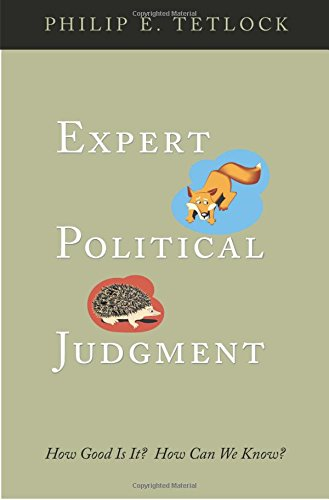
\includegraphics[height=0.7\textheight]{figures/tetlock_expert_2005_cover}
\end{center}

\vfill
20 years in the making

\end{frame}
%%%%%%%%%%%%%%%%%%%%%%%%%%%
\begin{frame}

\begin{center}
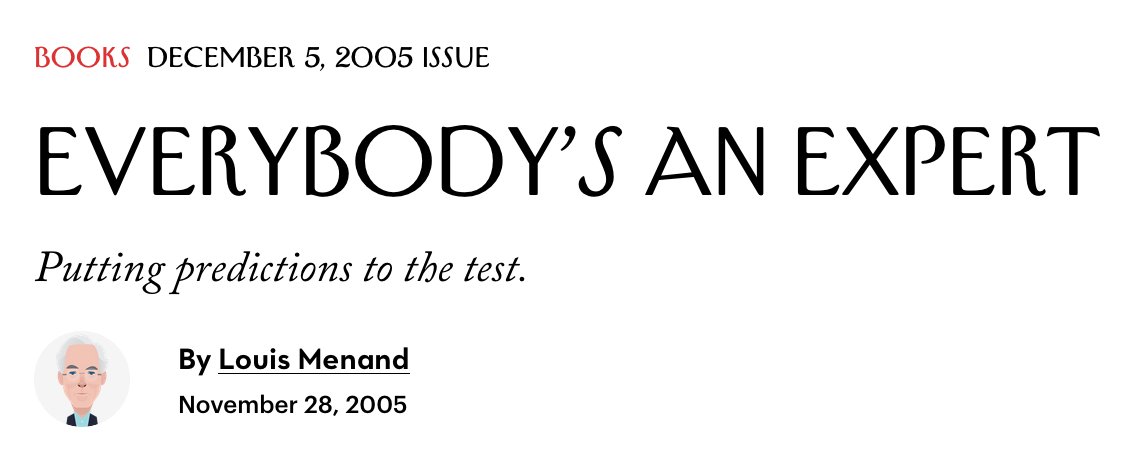
\includegraphics[width=0.9\textheight]{figures/menand_everybodys_2005_title}
\end{center}

\vfill
\url{https://www.newyorker.com/magazine/2005/12/05/everybodys-an-expert}

\end{frame}
%%%%%%%%%%%%%%%%%%%%%%%%%%%
\begin{frame}

\begin{center}
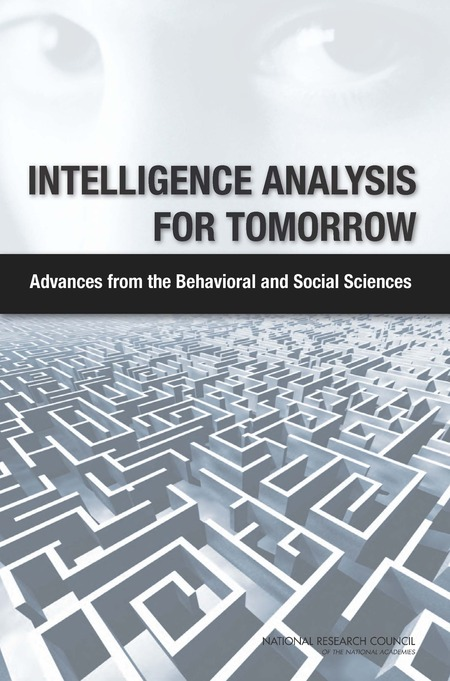
\includegraphics[height=0.7\textheight]{figures/nas_intellegence_2011_cover}
\end{center}

\vfill
\url{https://doi.org/10.17226/13040}

\end{frame}
%%%%%%%%%%%%%%%%%%%%%%%%%%%
\begin{frame}

\begin{center}
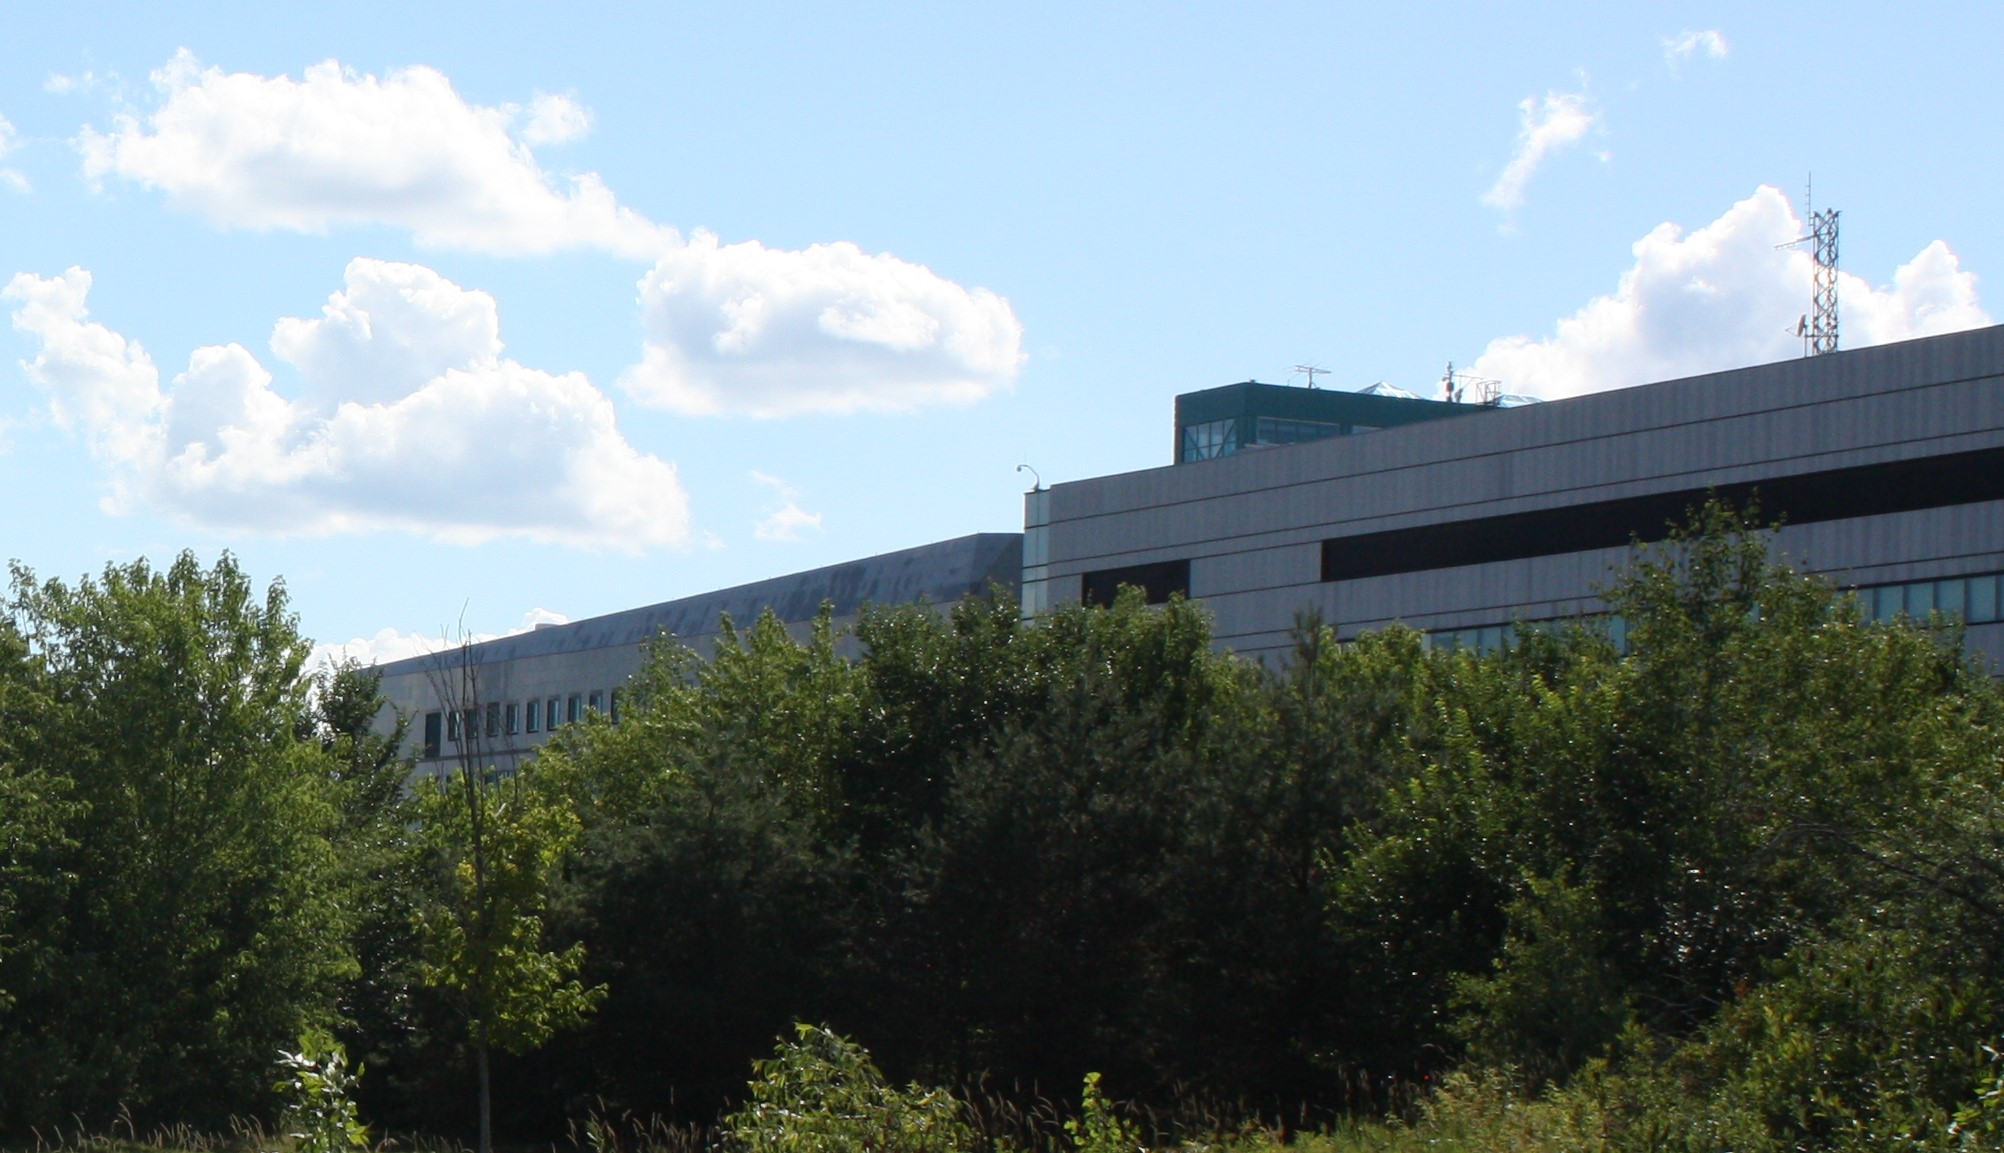
\includegraphics[width=\textwidth]{figures/CSIS_Ottawa_Building_Ogilvie_Canadian_Security_Intelligence_Service_(50182903412)}
\end{center}

\vfill
Intelligence Assessment Secretariat, part of the Canadian Security Intelligence Service
\end{frame}
%%%%%%%%%%%%%%%%%%%%%%%%%%
\begin{frame}

\begin{center}
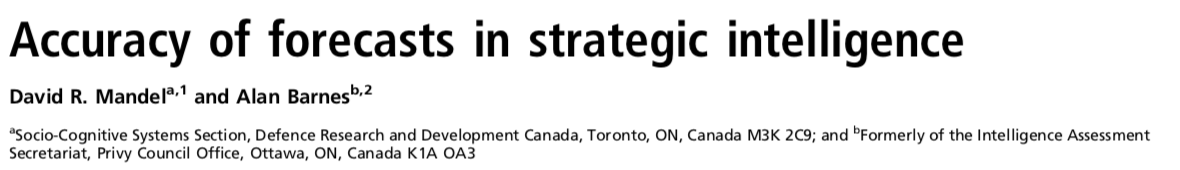
\includegraphics[width=\textwidth]{figures/mandel_accuracy_2014_title}
\end{center}

\vfill
\url{https://doi.org/10.1073/pnas.1406138111}

\end{frame}
%%%%%%%%%%%%%%%%%%%%%%%%%%%
\begin{frame}

Predictions embedded in reports:
\begin{itemize}
\item ``The intense distrust that exists between Country X and Country Y is almost certain [9/10] to prevent the current relationship of convenience from evolving into a stronger alliance.''
\item ``It is very unlikely [1/10] that either of these countries will make a strategic decision to launch an offensive in the coming six months.''
\end{itemize}

\end{frame}
%%%%%%%%%%%%%%%%%%%%%%%%%%%
\begin{frame}

Reading notes:
\begin{itemize}
\item How does the accuracy of these predictions compare to those in Tetlock?
\pause
\item What are the similarities and differences between the tasks in the two studies? 
\pause
\item Note: Tetlock (2005): roughly 15\% of cases had ambiguous outcomes (p 296), Mandel and Barnes (2014): 20\% of cases had ambiguous outcomes (p 10987)
\end{itemize}

\end{frame}
%%%%%%%%%%%%%%%%%%%%%%%%%%%
\begin{frame}

\begin{center}

\includegraphics[width=\textwidth]{figures/tetlock_judging_2014_title}
\end{center}

\vfill
\url{https://doi.org/10.1073/pnas.1412524111}

\end{frame}
%%%%%%%%%%%%%%%%%%%%%%%%%%
\begin{frame}

Reading notes
\begin{itemize}
\item How do they explain any difference in findings between Mandel and Barnes and Teltock (1995) and Mellers and Tetlock (comes after Tetlock 1995)?
\pause
\item What does this mean for our ability to learn anything from an empirical study like this?
\end{itemize}

\end{frame}
%%%%%%%%%%%%%%%%%%%%%%%%%%
\begin{frame}

\begin{center}
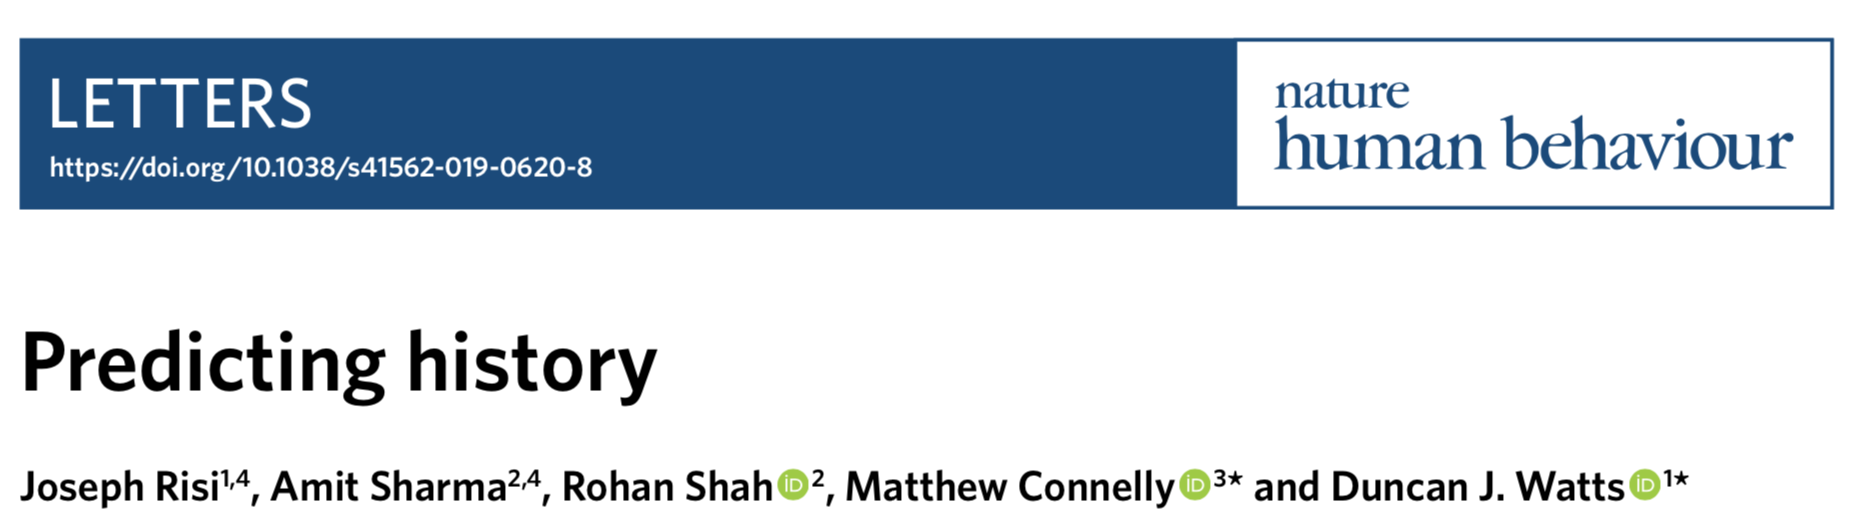
\includegraphics[width=\textwidth]{figures/risi_predicting_2019_title}
\end{center}

\vfill
\url{https://doi.org/10.1038/s41562-019-0620-8}

\end{frame}
%%%%%%%%%%%%%%%%%%%%%%%%%%
\begin{frame}

\begin{center}
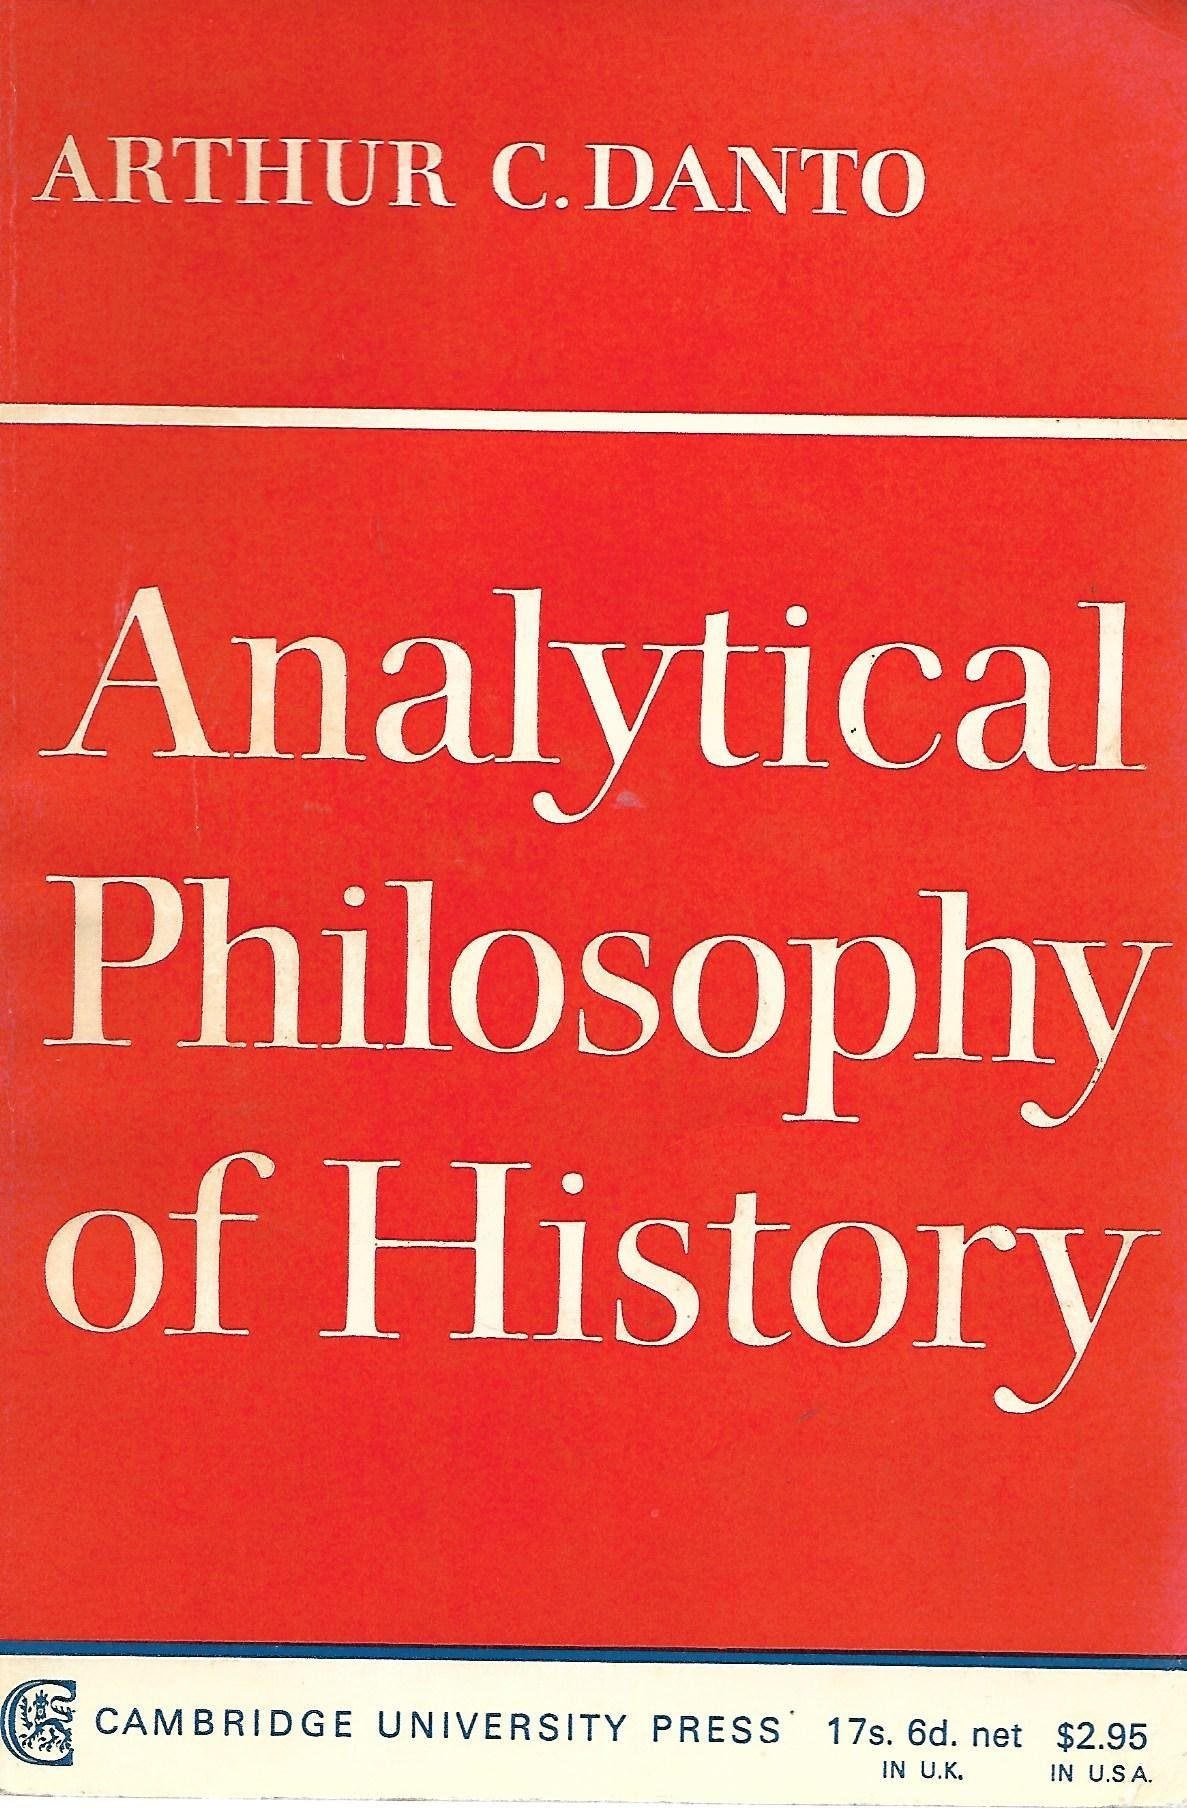
\includegraphics[height=0.8\textheight]{figures/danto_analytical_1965_cover}
\end{center}

\note{
Let's think about the events that we now consider to be historic.  Some of these were clearly seen as historic at that time.  Fall of the Berlin Wall.  Some events that we now think of as historic were not widely seen that way at the time.  For example, the first confirmed case of HIV/AIDS in the US is now considered historically important in the US, but that was not clear at the time.  And sometimes there are thought to be historic today, but are forgotten (many examples from politics and sports).

Is it even possible to know now what events will come to be considered historically important?

Danto proposes a thought experiment: the ideal chronicler.

``Danto imagined a hypothetical entity—the ideal chronicler—that possesses complete information about the state of the world, along with its entire history up to that point, and unlimited ability to integrate and analyse that information. Danto then argued that the ideal chronicler would still be unable to anticipate the significance that will be assigned to contemporaneous events by future historians because their judgements are inevitably informed by events that have not yet taken place. Evaluating the historical significance of a single event would in principle require the ideal chronicler to accurately predict not only its impact on subsequent events, but also how those events would impact broader social structures and practices. For example, to have anticipated the historical significance of the storming of the Bastille on 14 July 1789, the ideal chronicler would have had to predict not only the whole sequence of events leading to the French Revolution, but also their transformation of political and philosophical notions of sovereignty—a profound structural shift that has arguably shaped all subsequent revolutionary movements.''

}
\end{frame}
%%%%%%%%%%%%%%%%%%%%%%%%
\begin{frame}

All US State Department Cables (1973-1979). About 2 million cables of which about 2 thousand (~1 in 1,000) were judged to be historically significant.
\pause

\begin{center}
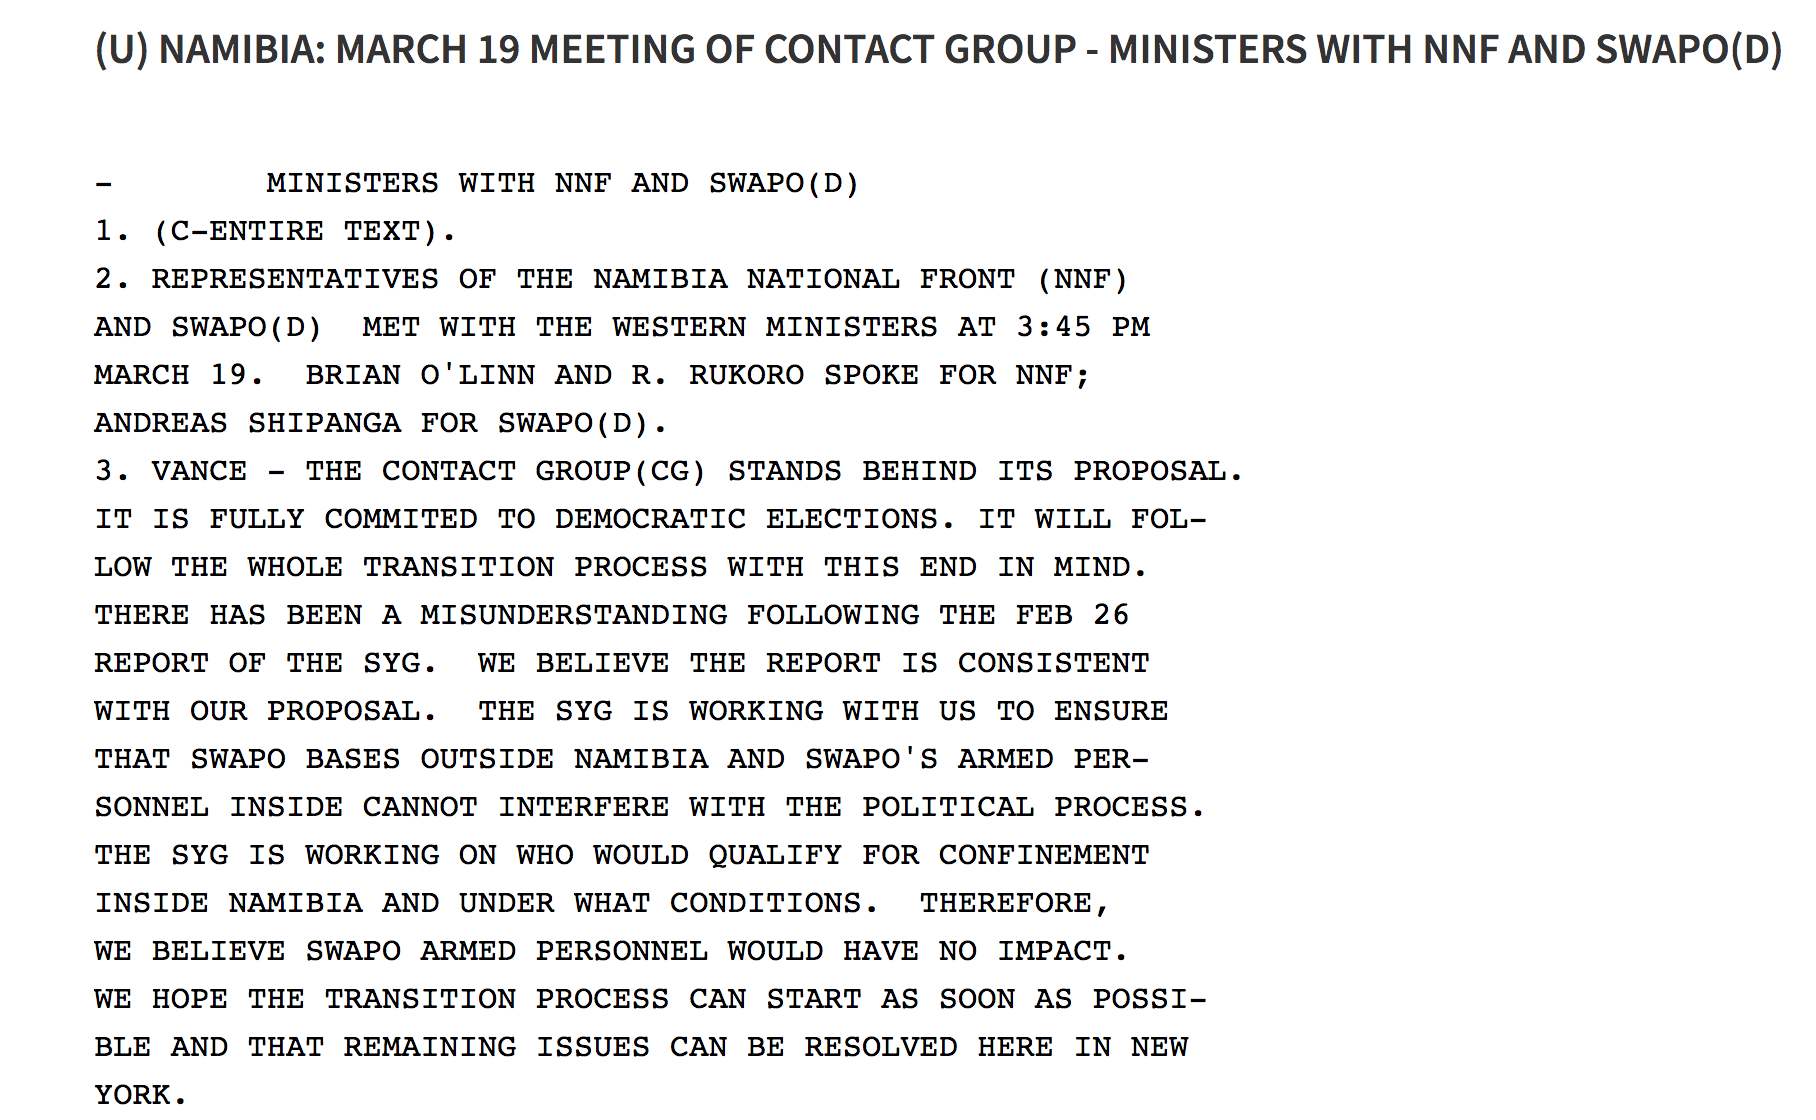
\includegraphics[height=0.5\textheight]{figures/cable_1979SECTO03013}
\end{center}

\vfill

\tiny{\url{http://history-lab.org/documents/1979SECTO03013}}

\end{frame}
%%%%%%%%%%%%%%%%%%%%%%%%%
\begin{frame}

Reading notes:
\begin{itemize}
\item We see new measures of performance: precision, recall, and F1 score. If you are not familiar with these read the Methods section carefully because we will see these again.
\pause
\item How accurately can the perceived contemporaneous impression of importance judgements predict subsequent judgement by historians?
\pause
\item How well can an ML model trained on the full cables predict subsequent judgement by historians?
\pause
\item What do the errors of both approaches teach us?
\pause 
\item Overall, what do these results suggest for Danto's argument about the ideal chronicler?
\end{itemize}

\end{frame}
%%%%%%%%%%%%%%%%%%%%%%%%%
\begin{frame}

\begin{center}
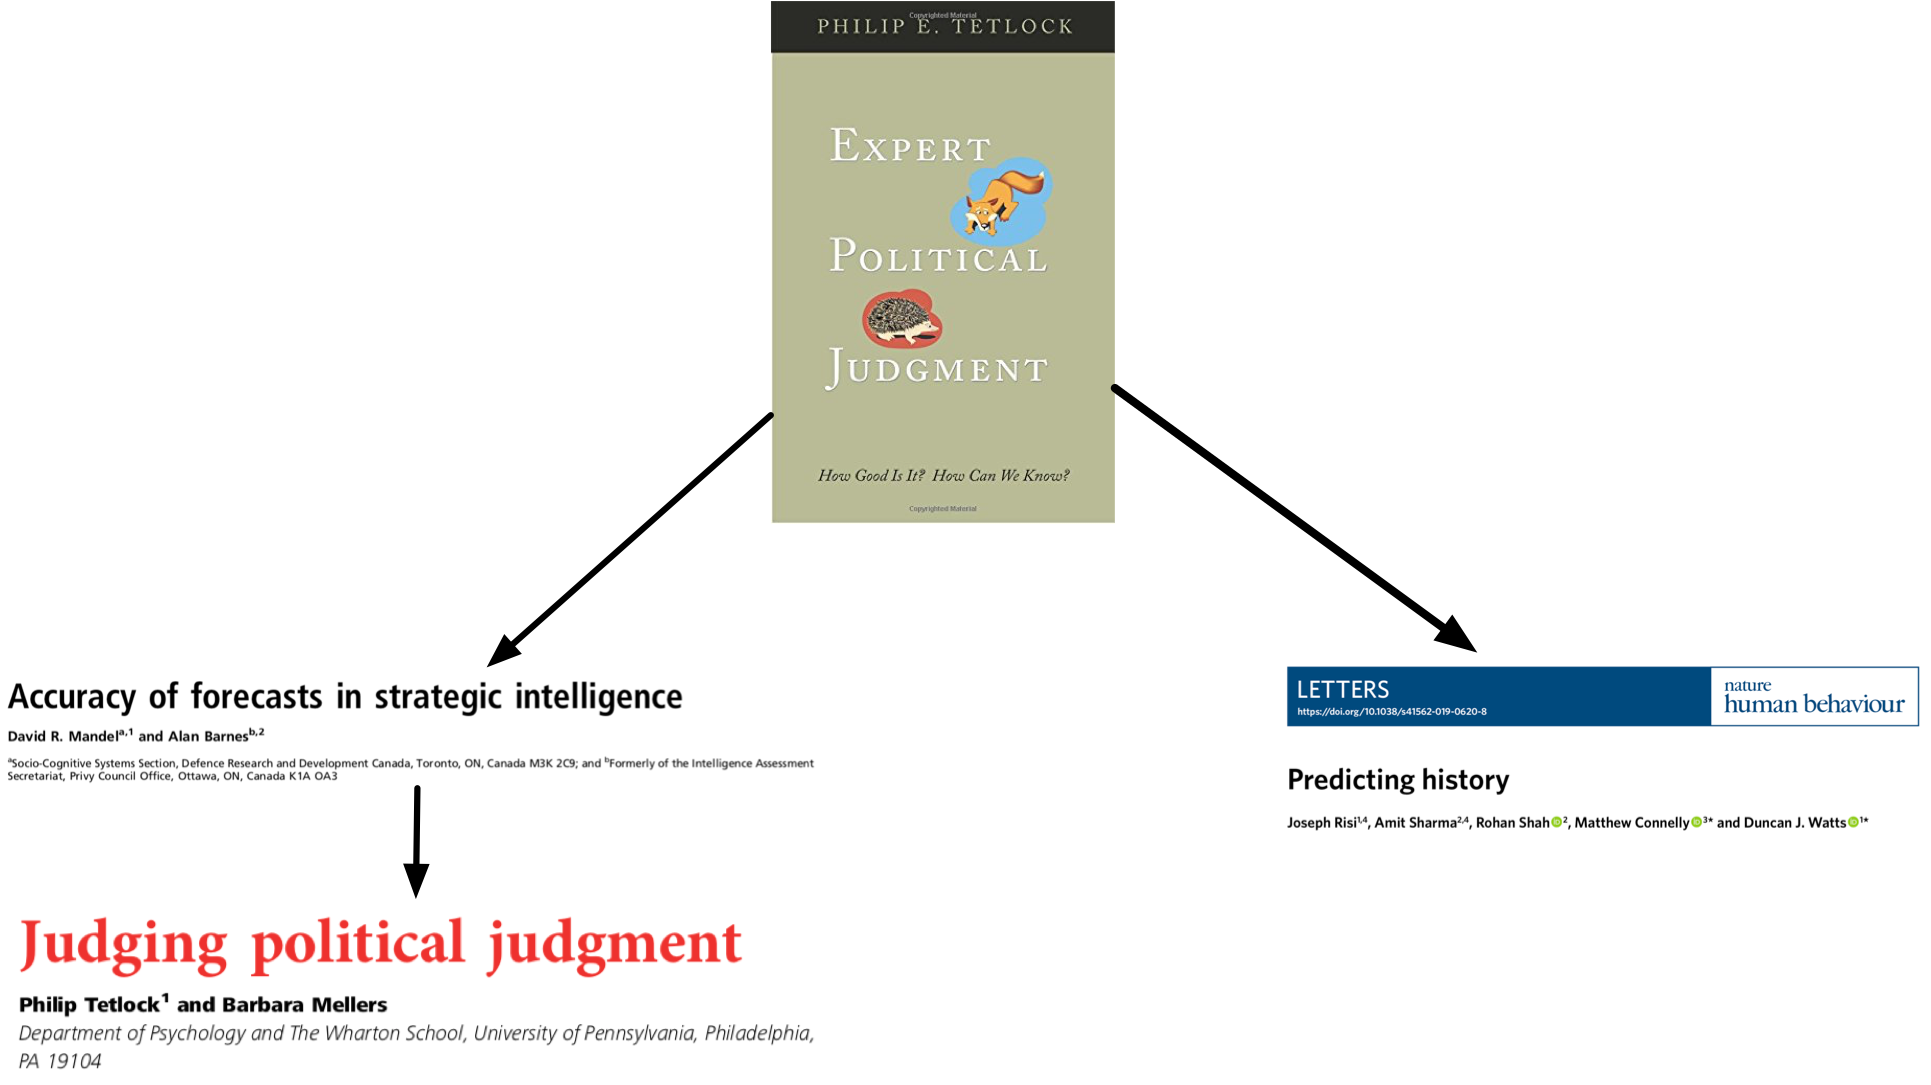
\includegraphics[height=0.6\textheight]{figures/geopolitical_ideamap}
\end{center}

\end{frame}
%%%%%%%%%%%%%%%%%%%%%%%%
\begin{frame}

\begin{center}
\LARGE{Additional thoughts}
\end{center}

\end{frame}
%%%%%%%%%%%%%%%%%%%%%%%%%%
\begin{frame}

Overconfidence without confidence intervals \pause
\begin{itemize}
\item Normally, when we produce an estimate we need to produce a confidence interval.  In this case underconfidence, is having confidence intervals that are too big.
\pause
\item In Mandel and Barnes, analysts don't produce confidence intervals but they still talk about underconfidence.
\pause
\item Is there a role for confidence intervals (sometimes called predictive intervals) here? Would making accurate predictive intervals require understanding the mechanisms that lead to uncertainty  . . . and hence the limits of prediction?
\end{itemize}

\end{frame}
%%%%%%%%%%%%%%%%%%%%%%%%%%
\begin{frame}

What is hard what is easy?
\begin{itemize}
\item Tetlock and Mellers: ``We should, however, focus on the core problem that neither past nor current work has yet solved: how best to measure the deceptively simple concept of accuracy. \pause One challenge is that the standardization of difficulty.  Getting a good Brier score by predicting weather in a low-variance world (eg, Phoenix) is a lot easier than it is in a high-variance world (eg, St. Louis).''
\pause
\item Mandel and Barnes have a non-statistical way of thinking about difficulty (based on information base, number of factor, role for irrationality, time frame), see SI
\pause 
\item Mandel and Barnes did not provide a measure of  inter-coder reliability
\pause
\item Is there some way to use these expert created measures of difficulty to learn about the limits of prediction?
\end{itemize}

\end{frame}
%%%%%%%%%%%%%%%%%%%%%%%%%
\begin{frame}

What to read next:
\begin{itemize}
\item ``Bobby W.'' (2019) \href{https://www.cia.gov/library/center-for-the-study-of-intelligence/csi-publications/csi-studies/studies/vol-63-no-4/Limits-of-Prediction.html}{The Limits of Prediction---or How I Learned to Stop Worrying About Black Swans and Love Analysis} ``The key struggle for intelligence analysts is that they are made to produce and what their consumers think they can produce are often two different things.''
\item What to read next from last class
\end{itemize}

\end{frame}
%%%%%%%%%%%%%%%%%%%%%%%%%%%

\end{document}
